\documentclass{article}
\usepackage{mysettings}

\title{Relazione Progetto di Machine Learning \\Classificazione di lettere dell'alfabeto ASL}
\author{Habasescu Alin Marian}

\begin{document}

\maketitle

\tableofcontents
\clearpage

\section{Descrizione del Progetto}

L'obiettivo di questo progetto è progettare un sistema di classificazione in 
grado di identificare lettere statiche dell'alfabeto americano dei segni (ASL) a partire da immagini 
di dimensione \(28\times28\) pixel. Le lettere \(Y\) e \(Z\) sono escluse dall'analisi poichè 
richiedono movimento per essere rappresentate. 

Sono stati considerati e confrontati diversi modelli di Machine Learning affrontati durante il corso, al fine 
di identificare il modello che ottiene i migliori risultati in termini di accuratezza e capacità di generalizzazione.

\begin{itemize}
    \item \textbf{Naive Bayes}
    
    \item \textbf{Multi Layer Perceptron Classifier (MLPClassifier)}
    
    \item \textbf{Support Vector Machine (SVM)}
    
    \item \textbf{Decision Tree}
\end{itemize}

\paragraph{Metodologia}
Il progetto segue i seguenti passi principali: 
\begin{enumerate}
    \item  \textbf{Caricamento e visualizzazione dei dati}.
    \item  \textbf{Preprocessing dei dati}.
    \item  \textbf{Addestramento dei modelli} e \textbf{valutazione dei modelli}.
    \item  \textbf{Analisi dei Risultati ottenuti}.
\end{enumerate}

\section{I Dataset}

Nel progetto si utilizzano due dataset distinti per l'addestramento e la valutazione dei modelli. 
I dataset vengono caricati dai file CSV forniti tramite la funzione \textbf{load\_datasets}, che suddivide i dati 
in \textit{features} (valori dei pixel delle immagini) e \textit{target} (le lettere corrispondenti).

Il dataset di training è composto da 27455 campioni, mentre il dataset di test contiene 7172 campioni. 
Ogni campione rappresenta un'immagine di una lettera statica dell'alfabeto ASL, accompagnata dai valori di 
grigio relativi ai 784 pixel che costituiscono l'immagine.

La funzione \textbf{visualize\_dataset} consente di analizzare i dati caricati, mostrando un'anteprima grafica delle 
prime osservazioni sotto forma di immagini \(28\times28\) pixel in scala di grigi e associandole alle lettere 
dell'alfabeto ASL (0\-25, mappati su A\-Z).

\begin{figure}[H]
    \centering
    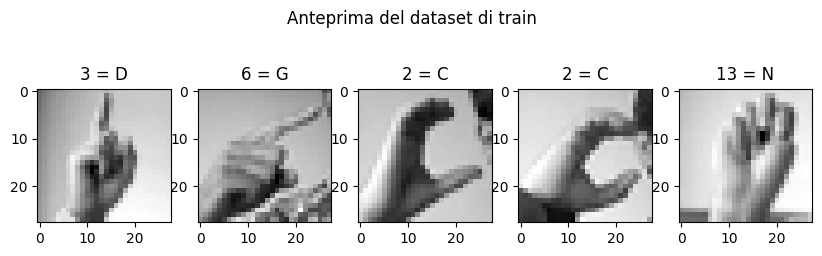
\includegraphics[scale=0.5]{Figures/output.png}\label{fig:dataset}
\end{figure}

\begin{figure}[H]  
    \centering
    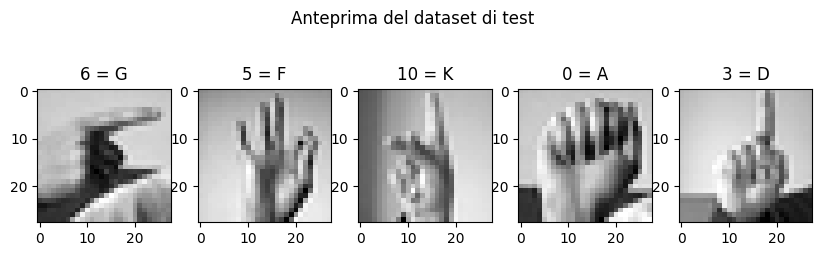
\includegraphics[scale=0.5]{Figures/output1.png}\label{fig:dataset_test}
\end{figure}

\clearpage

\section{Analisi Esplorativa dei Dati (EDA)}

Dopo il caricamento dei dataset, viene eseguita una serie di operazioni per analizzare le caratteristiche dei dati. 
La funzione \textbf{perform\_eda} viene utilizzata per eseguire l'analisi esplorativa dei dati.

\begin{itemize} 
    \item \textbf{Distribuzione delle classi}: Verifica di un bilanciamento uniforme tra le classi. 
    \item \textbf{Distribuzione dei valori dei pixel}: Analisi della gamma di valori di pixel (0\-255) per 
    determinare la necessità di normalizzazione. 
\end{itemize}

\begin{figure}[H]
    \centering
    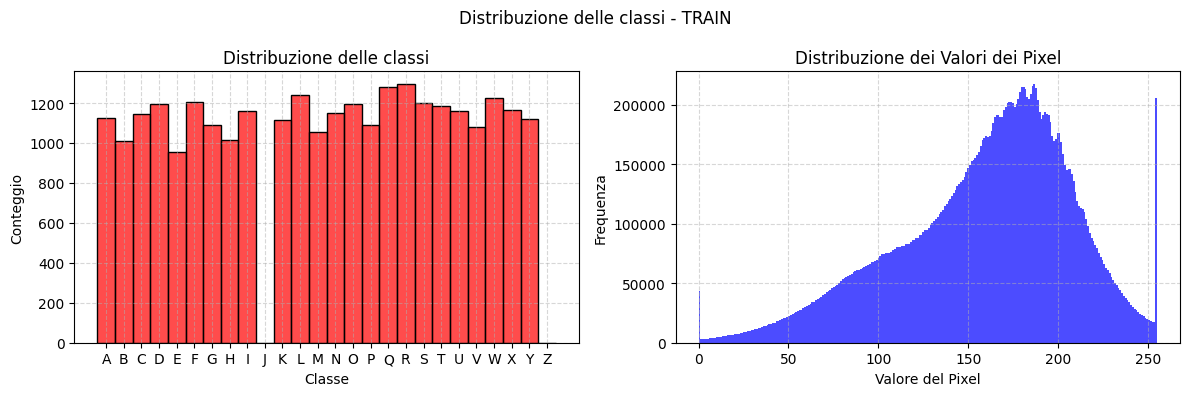
\includegraphics[scale=0.5]{Figures/output2.png}\label{fig:dataset_EDA}
\end{figure}

Durante l'analisi esplorativa dei dati, non sono stati osservati evidenti squilibri nella distribuzione delle classi 
del dataset di training. Sono stati trovati due picchi [0, 255] nel grafico della distribuzione dei valori dei pixel,
attribuibili ai valori di pixel molto bassi (0) e molto alti (255), rispettivamente. 

\section{Preprocessing dei dati}

Il preprocessing è stato fatto in due fasi principali:

\subsection{Standardizzazione}
I dati sono stati standardizzati utilizzando \texttt{StandardScaler} di scikit-learn, che 
\textbf{normalizza i dati in modo che abbiano media 0 e varianza 1}.

Questo processo è fondamentale per: 
\begin{itemize}
    \item Normalizzare la scala dei pixel 
    \item Migliorare la convergenza dei modelli
    \item Garantire che tutti i pixel contribuiscano euquivalentemente alla classificazione
\end{itemize}

\begin{figure}[H]
    \centering
    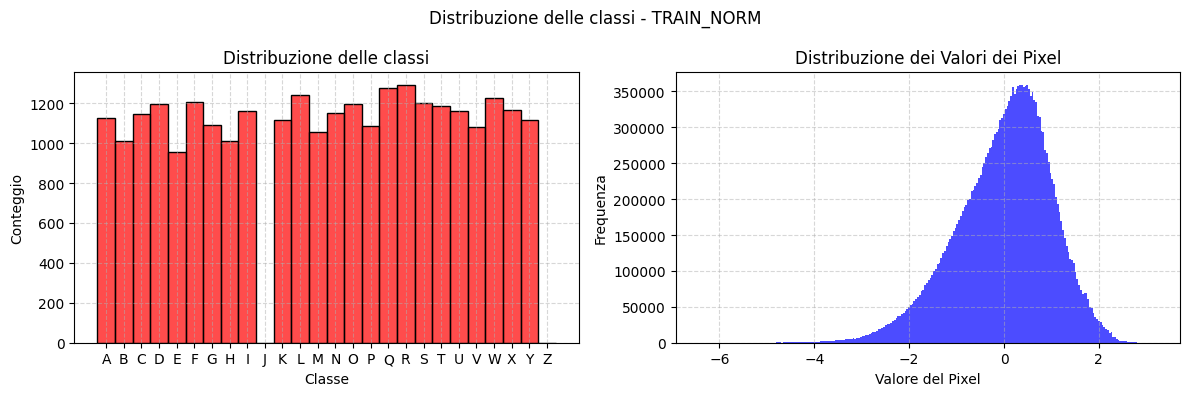
\includegraphics[scale=0.5]{Figures/output8.png}\label{fig:dataset_preprocessing}
\end{figure}

\subsection{Riduzione della dimensionalità}
E' stata applicata l'analisi delle componenti principali (PCA) per:
\begin{itemize}
    \item Riduzione della dimensionalità dei dati mantenendo il 95\% della varianza
    \item Diminuire il rumore nei dati
    \item Migliorare l'efficienza computazionale in generale
\end{itemize}

\clearpage

\section{Addestramento dei modelli e metriche di valutazione}

Sono stati implementati e confrontati quattro modelli di Machine Learning ciascuno 
con caratteristiche specifiche: 

\subsection{Modelli Implementati}

\begin{itemize}
    \item \textbf{Naive Bayes}: Un modello di classificazione probabilistico che fa uso del 
    Teorema di Bayes e dell'indipendenza tra le features.  
    
    \item \textbf{MLPClassifier}: Una rete neurale a più strati con le seguenti caratteristiche
    
        \begin{itemize}
            \item Architettura: tre layer nascosti (256, 128, 64 neuroni)
            \item Funzione di attivazione ReLU
            \item Ottimizzatore: Adam
            \item Numero massimo di iterazioni: 5000
            \item Regolarizzazione L2 con \texttt{alpha=0.0001}
        \end{itemize}

    \item \textbf{Support Vector Machine (SVM)}: Un algoritmo di classificazione che trova un iperpiano 
    ottimale che separa le classi. In questo progetto, l'algoritmo SVM utilizza il kernel Radial Basis 
    Function (RBF) per proiettare i dati in uno spazio di alta dimensionalità e trovare l'iperpiano 
    di separazione.
    
    \item \textbf{Decision Tree}: Un modello basato su una struttura ad albero, che suddivide i dati in 
    base a regole decisionali sequenziali, fino a profondità massiama di 25. 
\end{itemize}

\paragraph{Metriche di valutazione}

Per valutare le performance dei modelli sono state utilizzate le seguenti metriche di valutazione: 
\begin{itemize}
    \item \textbf{Accuracy}: Rappresenta la percentuale di campioni correttamente classificati.
    \item \textbf{F1\_score}: \[F1 = 2 \cdot \frac{\text{Precision} \cdot 
                                    \text{Recall}}{\text{Precision} + \text{Recall}}\]
    Media armonica tra precision\footnote{La percentuale di esempi correttamente 
    classificati rispetto a tutti quelli predetti per una certa classe} e recall\footnote{La percentuale di 
    esempi correttamente classificati rispetto a tutti i veri esempi di una certa classe}
    \item \textbf{Classification Report}: Precision, Recall e F1-Score per ogni classe.
    \item \textbf{Confusion Matrix}: Matrice di confusione che mostra il numero di campioni correttamente 
    classificati per ogni classe.
\end{itemize}

I risultati sono stati confrontati tramite un grafico a barre che mostra le accuratezze dei modelli

\clearpage
\section{Risultati ottenuti}

L'analisi delle performance ha prodotto i seguenti risultati: 

\begin{figure}[H]
    \centering
    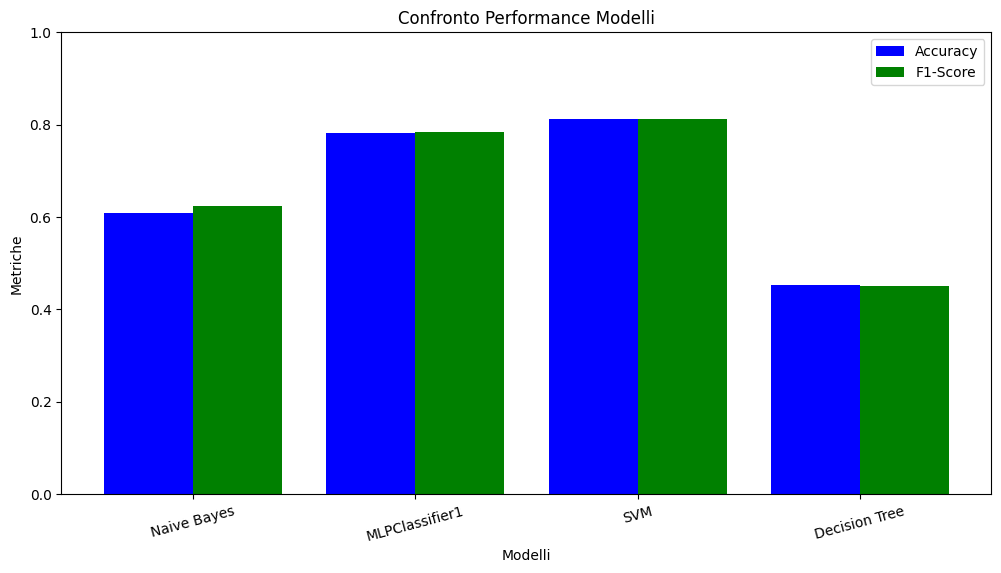
\includegraphics[scale=0.5]{Figures/output9.png}
\end{figure}

\begin{itemize}
    \item \textbf{Support Vector Machine (SVM)} ha ottenuto l'accuratezza migliore (86\%) tra i 
    modelli analizzati, sebbene con un alto costo computazionale. 
    Questo modello è stato particolarmente efficace nel trovare l'iperpiano ottimale grazie alla sua 
    capacità di lavorare in spazi ad alta dimensione. Tuttavia, la sua performance è stata limitata 
    dalla necessità di una grande quantità di risorse computazionali, rendendo la sua implementazione 
    meno pratica in scenari a larga scala.
    
    \item \textbf{MLPClassifier} ha raggiunto un'accuratezza dell'80\%, posizionandosi al secondo 
    posto. Il modello ha avuto successo grazie alla sua capacità di catturare pattern complessi 
    nelle immagini grazie alla struttura a più layer nascosti. 
    
    \item \textbf{Naive Bayes} ha ottenuto un'accuratezza del (60\%), principalmente a causa 
    dell'assunzione di indipendenza tra le features. 
    Questa ipotesi, non tiene conto che nelle immagini pixel vicini tendono ad avere valori di grigio simili.
    
    \item \textbf{Decision Tree} ha mostrato i risultati peggiori (43\%). 
    Il modello ha avuto difficoltà nel catturare pattern complessi, portando a performance 
    insoddisfacenti rispetto ad altri modelli più sofisticati. 
\end{itemize}

\end{document}
